\documentclass[11pt]{article}
\usepackage[utf8]{inputenc}
\usepackage{graphicx}
\usepackage{subfig}
\usepackage{enumerate}
\usepackage{fourier}
\usepackage{booktabs}
\usepackage[T1]{fontenc}
% \usepackage[letter,width=150mm, top=30mm, bottom=30mm]{geometry}
\usepackage[font={footnotesize}]{caption}
\usepackage[labelfont=bf]{caption}
\usepackage[english]{babel}
\usepackage{amsmath}
% \usepackage{fontspec}

\setlength{\parskip}{1em}
\graphicspath{{../figs/}}

\title{Practice Session 05: Brune Spectral Ratio}
\author{Prithvi Thakur}
\date{Mar 11, 2019}

\begin{document}

\maketitle

% Problem 1
\section*{Synthetic Spectral Ratio}
We construct a spectral ratio for for a frequency range of $3 - 200$ Hz and a moment ratio ($M_{01}/M_{02}$) of $100$. The corner frequencies are $fc_1 = 20$ Hz and $fc_2 = 50$ Hz.

The spectral ratio is given by:
\begin{equation}
    R = \frac{u_1(f)}{u_2(f)} = \frac{M_{01}}{M_{02}}\big(\frac{1 + (f/fc_2^2)}{1 + (f/fc_1^2)}\big)
\end{equation}

Here $R$ is the spectral ratio. The brune spectral ratio without noise is shown in Fig. 1. The synthetic spectral ratio with added uniformly distributed white noise with a peak amplitude of 5 is shown in Fig. 2

\begin{figure}[!htb]
    \centering
    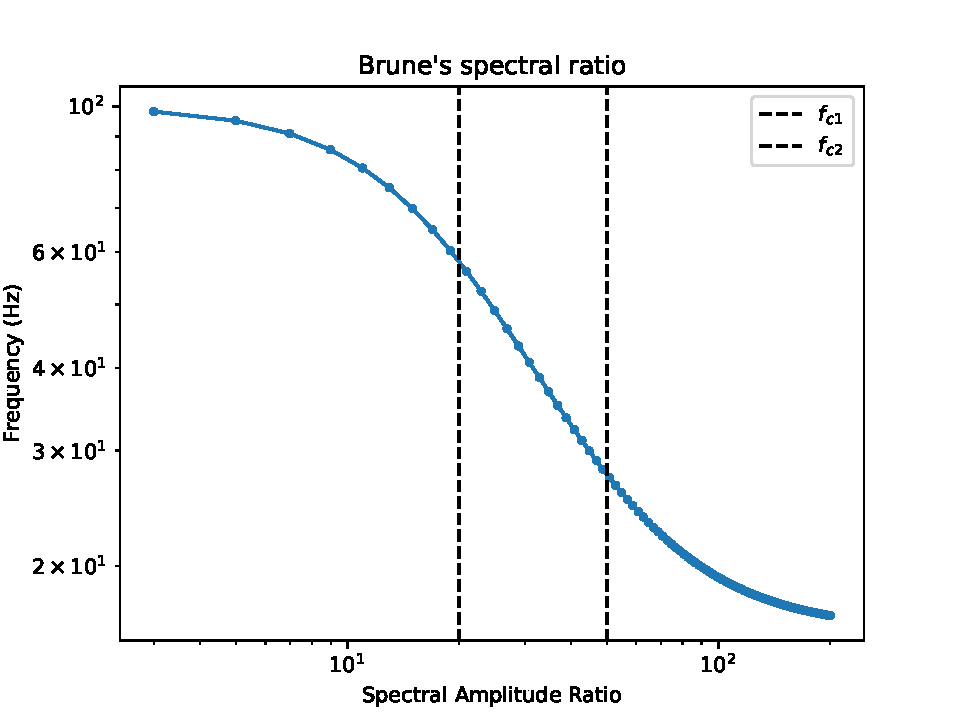
\includegraphics[scale=0.7]{fig1.pdf}
    \caption{Brune's spectral ratio without noise}
\end{figure}
\begin{figure}[!htb]
    \centering
    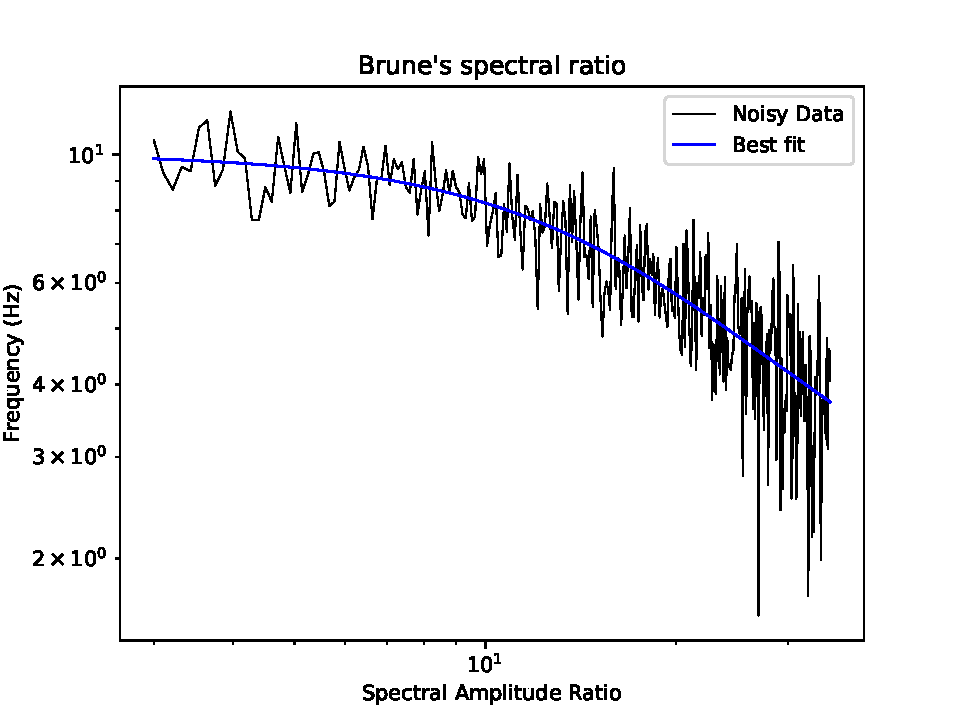
\includegraphics[scale=0.7]{fig_noise_1.pdf}
    \caption{Synthetic spectral ratio with noise peak amplitude of 5.}
\end{figure}
\clearpage

\section*{Best fit curve using the Brune's Model}
We use damped least squares to solve the nonlinear curve fitting, analogous to robustfit in Matlab. The best fit curve is shown in Fig. 3. The values of moment ratio and the corner frequencies are as follows (the superscript represents the noise level):

\begin{align*}
    &R^5 = 102.212 \\
    &fc_1^5 = 20.156 Hz \\
    &fc_2^5 = 47.474 Hz
\end{align*}
\begin{figure}[!htb]
    \centering
    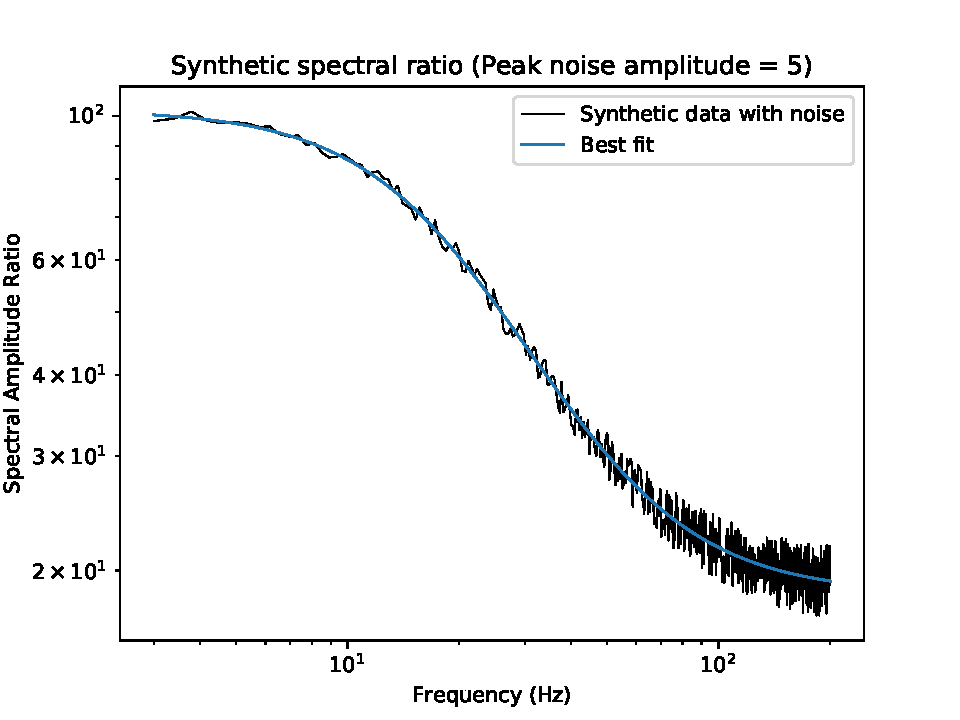
\includegraphics[scale=0.7]{fig_noise_2.pdf}
    \caption{Synthetic spectral ratio with noise peak amplitude of 5.}
\end{figure}

We get values of moment ratio and corner frequencies very close to the true values from inversion.

\section*{Increasing the amplitude of white noise}
We increase the peak noise amplitude and look at the inversion results. The results are shown in Fig. 4, 5, 6 and their values are shown below.
\begin{align*}
    &R^{10} = 104.444 \\
    &fc_1^{10} = 20.354 Hz \\
    &fc_2^{10} = 45.680 Hz
\end{align*}
\begin{figure}[!htb]
    \centering
    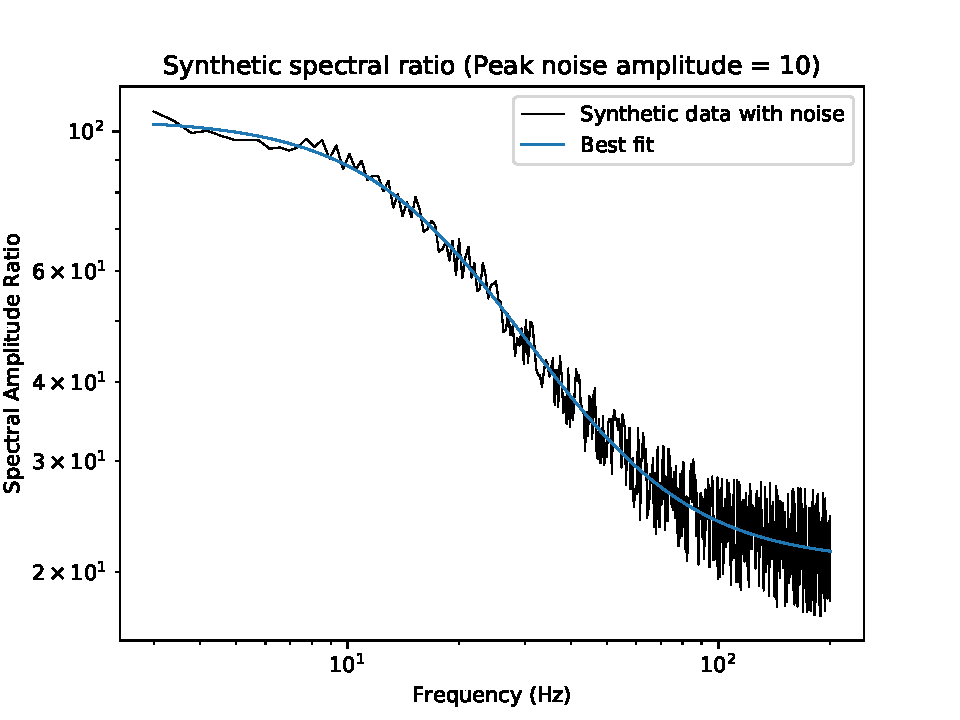
\includegraphics[scale=0.7]{fig_noise_3.pdf}
    \caption{Synthetic spectral ratio with noise peak amplitude of 10.}
\end{figure}
\begin{align*}
    &R^{20} = 110.330 \\
    &fc_1^{20} = 19.381 Hz \\
    &fc_2^{20} = 39.625 Hz
\end{align*}
\begin{figure}[!htb]
    \centering
    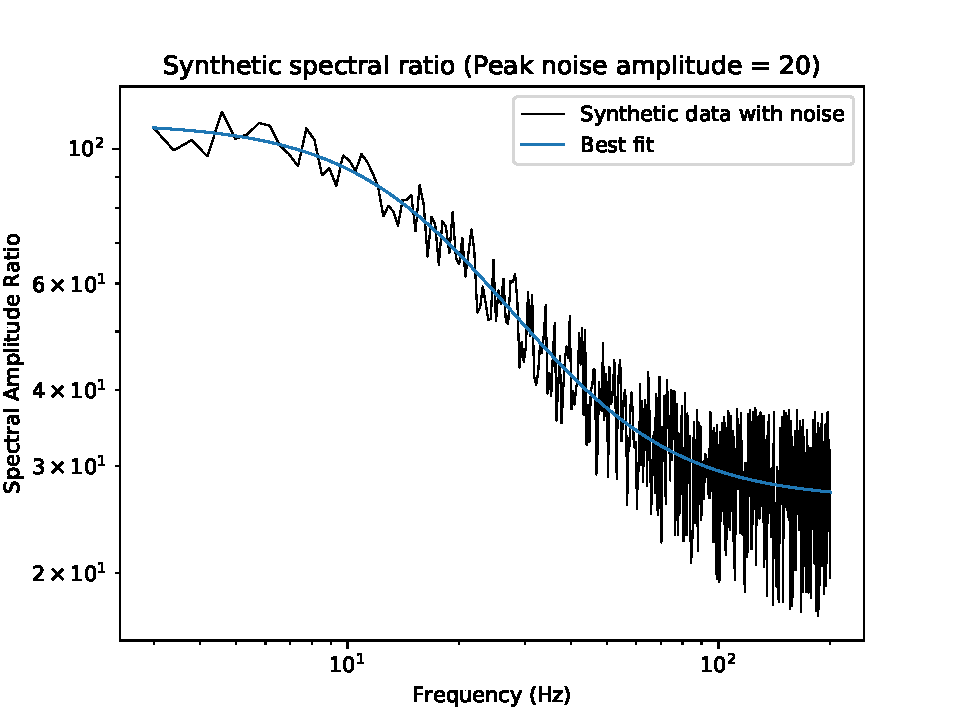
\includegraphics[scale=0.7]{fig_noise_4.pdf}
    \caption{Synthetic spectral ratio with noise peak amplitude of 20.}
\end{figure}
\begin{align*}
    &R^{50} = 125.009 \\
    &fc_1^{50} = 20.418 Hz \\
    &fc_2^{50} = 35.746 Hz
\end{align*}
\begin{figure}[!htb]
    \centering
    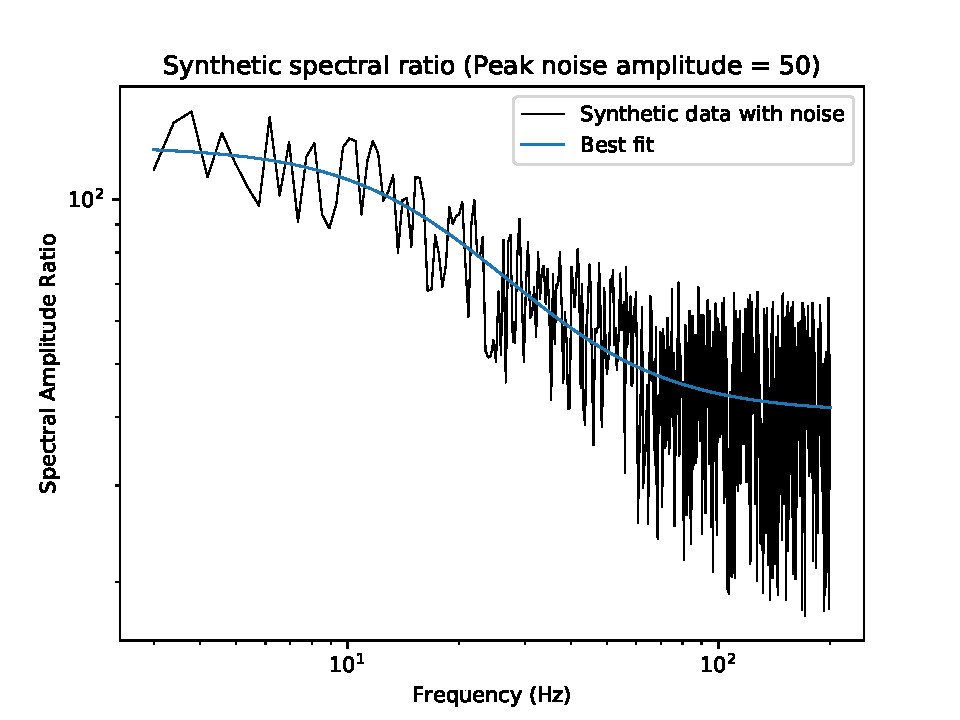
\includegraphics[scale=0.7]{fig_noise_5.pdf}
    \caption{Synthetic spectral ratio with noise peak amplitude of 50.}
\end{figure}

We see that we get increasing errors with increasing peak noise amplitude level but it scales linearly with increasing noise. The values of $fc_2$ are less robust to inversion than the moment ratio and $fc_1$. There is significant deviation in all the three values at peak noise amplitude of $50$ and above. 

\clearpage
\section*{Synthetic spectral ratio with limited frequency}
We cut the synthetic spectral ratio to a range of $3-35$ Hz and try the best fitting with peak noise levels of $5, 10, 20, 50$ and look at the inverted values below. The best fit curves are shown in Fig. 7, 8, 9, 10, and the values are listed in Table 1. We see that the moment ratio and the corner frequency $fc_1$ is better estimated than $fc_2$, because we have a limited frequency of data available.
\begin{center}
\begin{table}
    \begin{tabular}{l c c c}
        \toprule%
        Peak Noise Level & Moment Ratio & $fc_1$ & $fc_2$ \\
        \midrule
        \multicolumn{4}{c}{Frequency Range $3-200$ Hz, Moment Ratio 100}\\
        \midrule
        0 & 100 & 20 & 50 \\
        5 & 102.212 & 20.156 & 47.474 \\
        10 & 104.444 & 20.354 & 45.680\\
        20 & 110.330 & 19.381 & 39.625\\
        50 & 125.009 & 20.418 & 35.746\\
        \midrule
        \multicolumn{4}{c}{Frequency Range $3-35$ Hz, Moment Ratio 100}\\
        \midrule
        5 & 102.522 & 20.094 & 47.713 \\
        10 & 104.250 & 20.367 & 45.894\\
        20 & 111.088 & 19.818 & 40.999\\
        50 & 128.728 & 17.470 & 29.304\\
        \midrule
        \multicolumn{4}{c}{Frequency Range $3-35$ Hz, Moment Ratio 10}\\
        \midrule
        0 & 10 & 20 & 50 \\
        5 & 12.439 & 21.442 & 40.894 \\
        10 & 15.187 & 16.637 & 24.192\\
        20 & 21.622 & 13.665 & 17.351\\
        50 & 51.577 & 3.02 & 3.988\\
        \bottomrule
    \end{tabular}
    \caption{Inverted values for all the cases}
\end{table}
\end{center}

\begin{figure}[!htb]
    \centering
    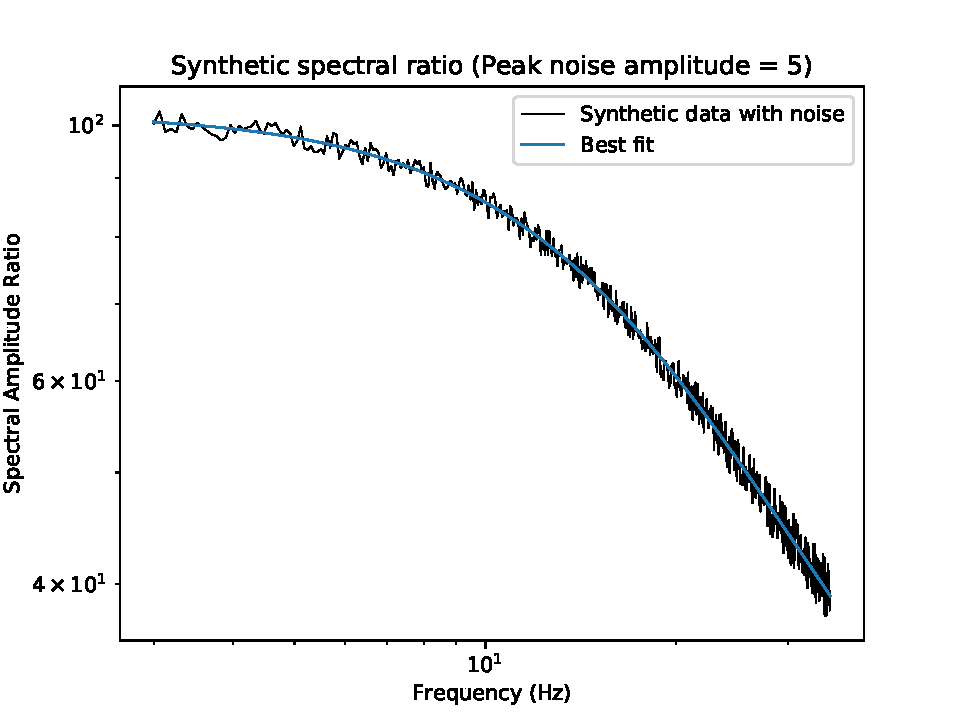
\includegraphics[scale=0.7]{fig_freq_noise_1.pdf}
    \caption{Synthetic spectral ratio with noise peak amplitude of 5.}
\end{figure}
\begin{figure}[!htb]
    \centering
    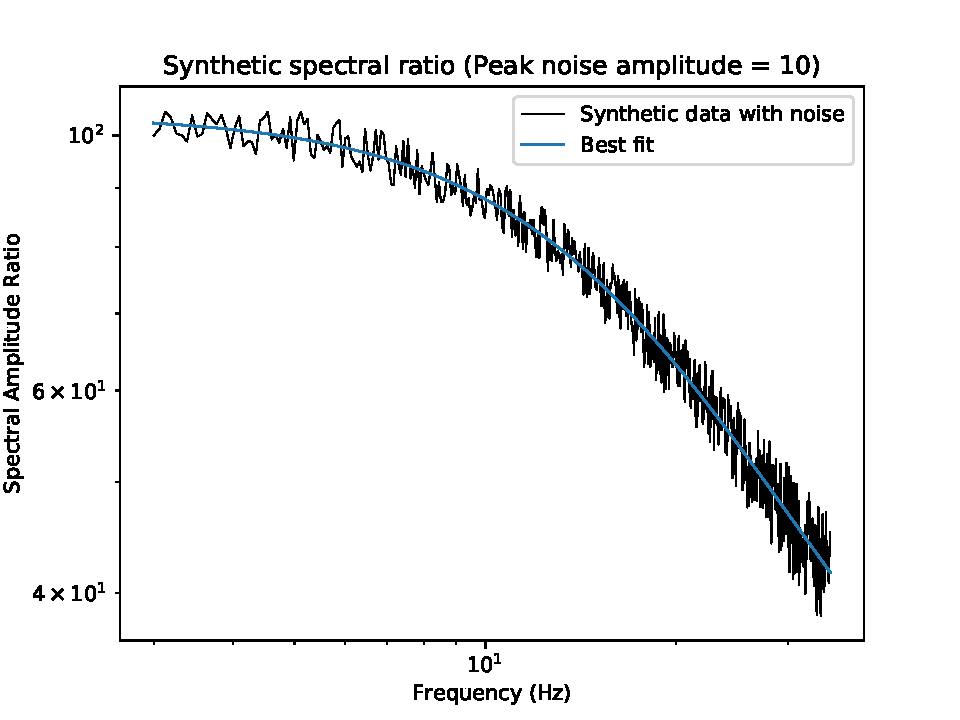
\includegraphics[scale=0.7]{fig_freq_noise_2.pdf}
    \caption{Synthetic spectral ratio with noise peak amplitude of 10.}
\end{figure}
\begin{figure}[!htb]
    \centering
    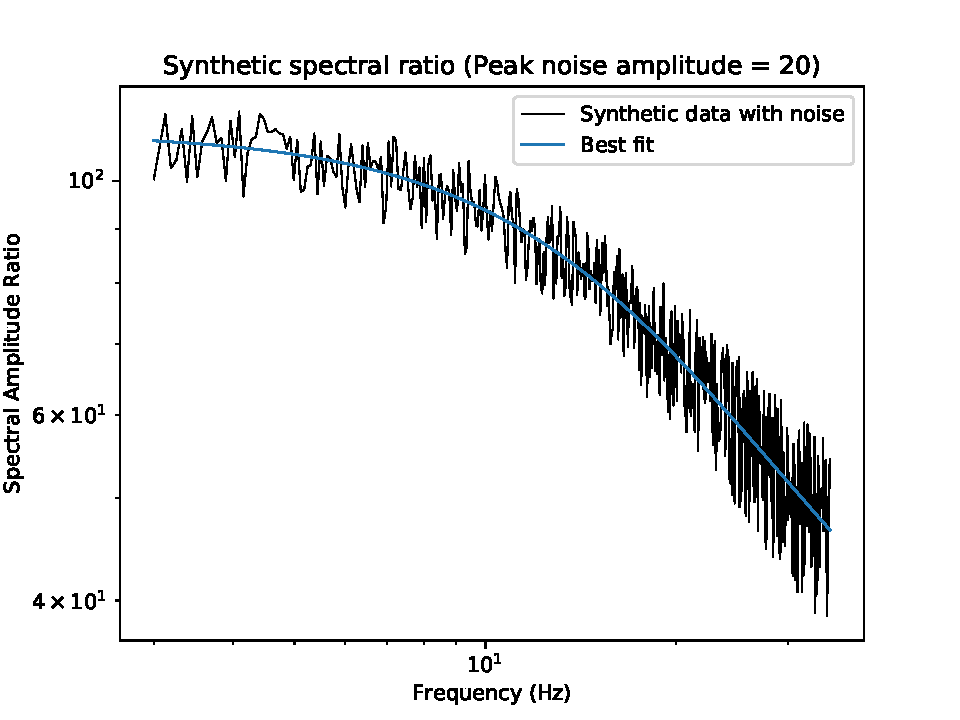
\includegraphics[scale=0.7]{fig_freq_noise_3.pdf}
    \caption{Synthetic spectral ratio with noise peak amplitude of 20.}
\end{figure}
\begin{figure}[!htb]
    \centering
    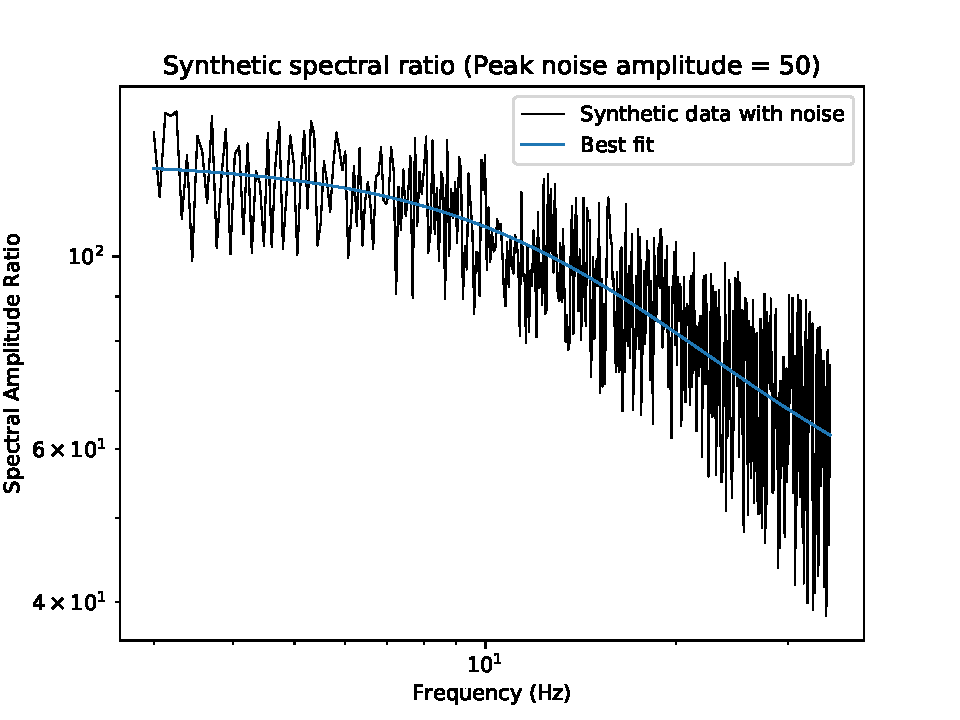
\includegraphics[scale=0.7]{fig_freq_noise_4.pdf}
    \caption{Synthetic spectral ratio with noise peak amplitude of 50.}
\end{figure}

In the next part, we change the moment ratio to 10 and see the response to increasing noise on the moment ratio and corner frequency inversion. Since the moment ratio is low, we see that any inversion with peak noise greater than 10 gives totally unreliable inversion results even for the corner frequencies (Fig, 11, 12, 13, 14). The inversions give the peak noise level as the output rather than the moment ratio of synthetic data.

\begin{figure}[!htb]
    \centering
    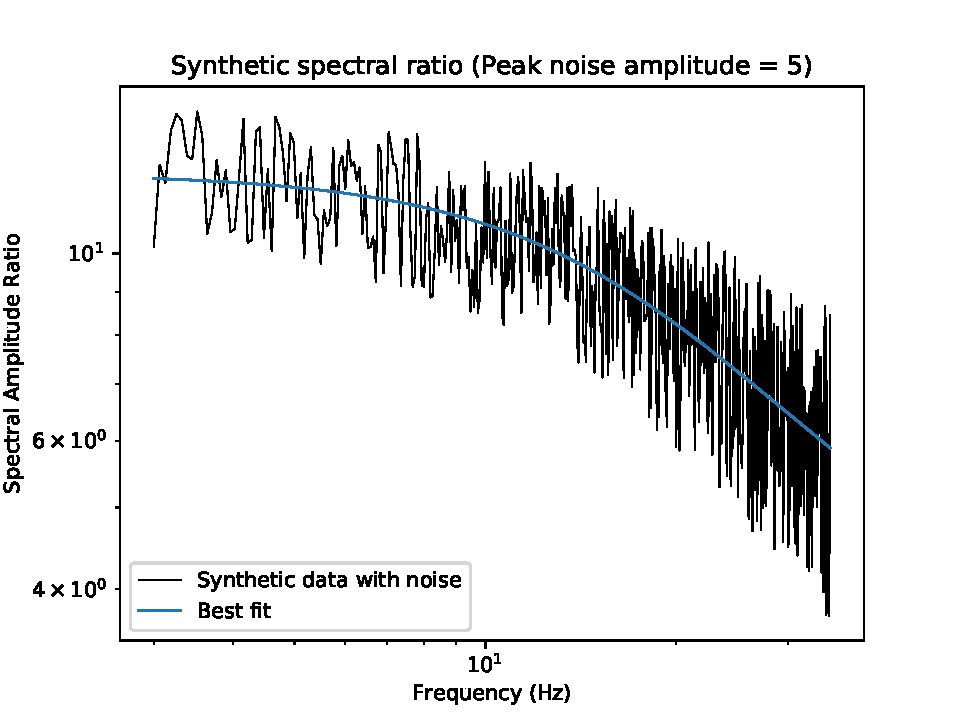
\includegraphics[scale=0.7]{fig_mom_noise_1.pdf}
    \caption{Synthetic spectral ratio with noise peak amplitude of 5.}
\end{figure}
\begin{figure}[!htb]
    \centering
    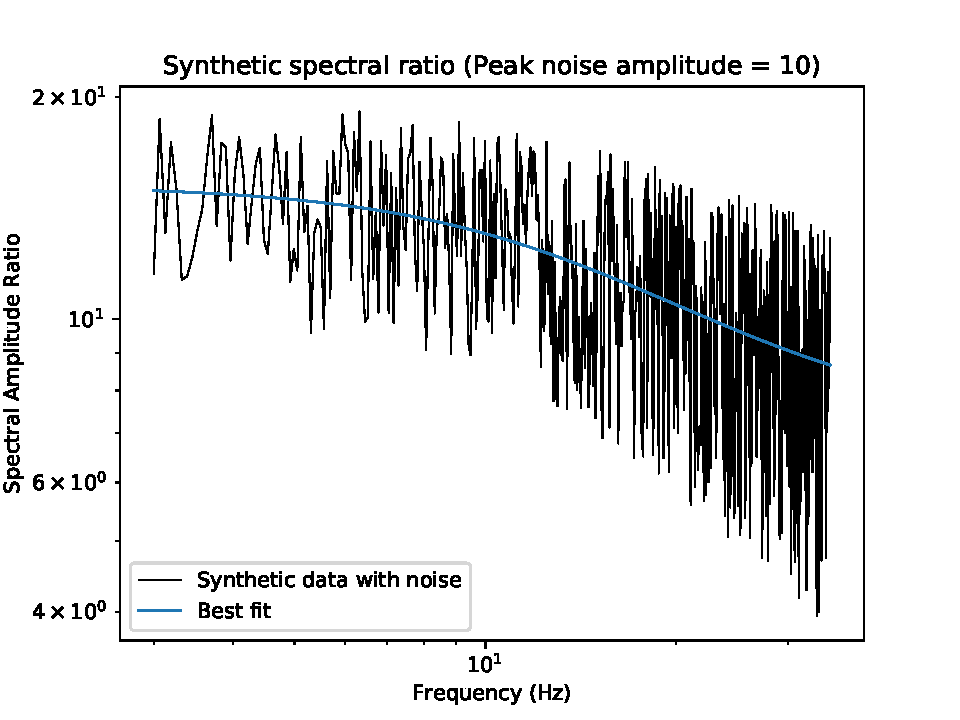
\includegraphics[scale=0.7]{fig_mom_noise_2.pdf}
    \caption{Synthetic spectral ratio with noise peak amplitude of 10.}
\end{figure}
\begin{figure}[!htb]
    \centering
    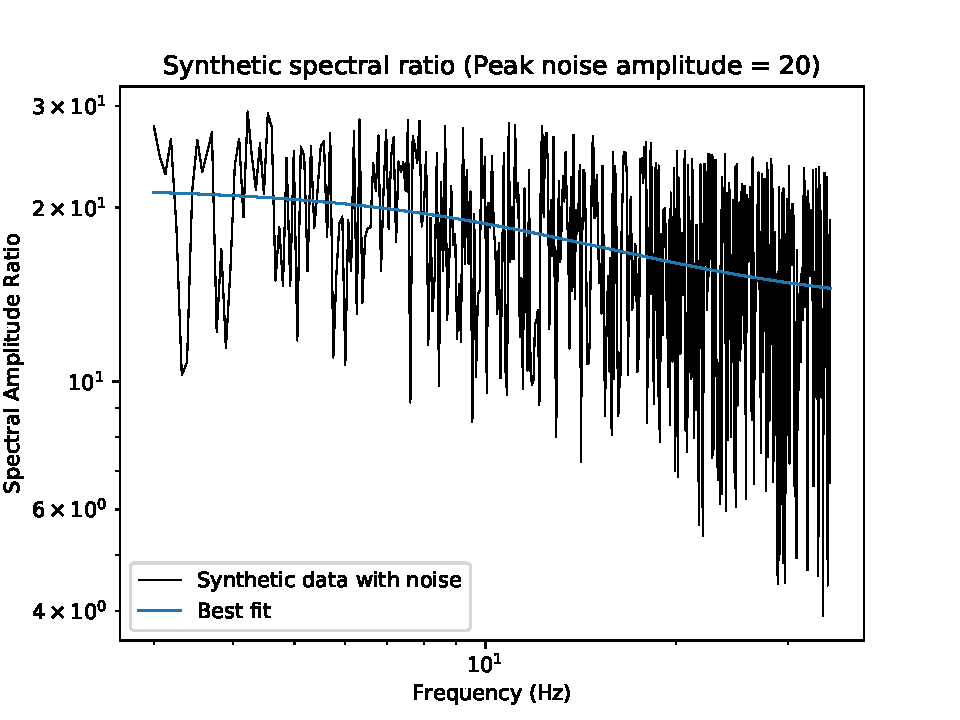
\includegraphics[scale=0.7]{fig_mom_noise_3.pdf}
    \caption{Synthetic spectral ratio with noise peak amplitude of 20.}
\end{figure}
\begin{figure}[!htb]
    \centering
    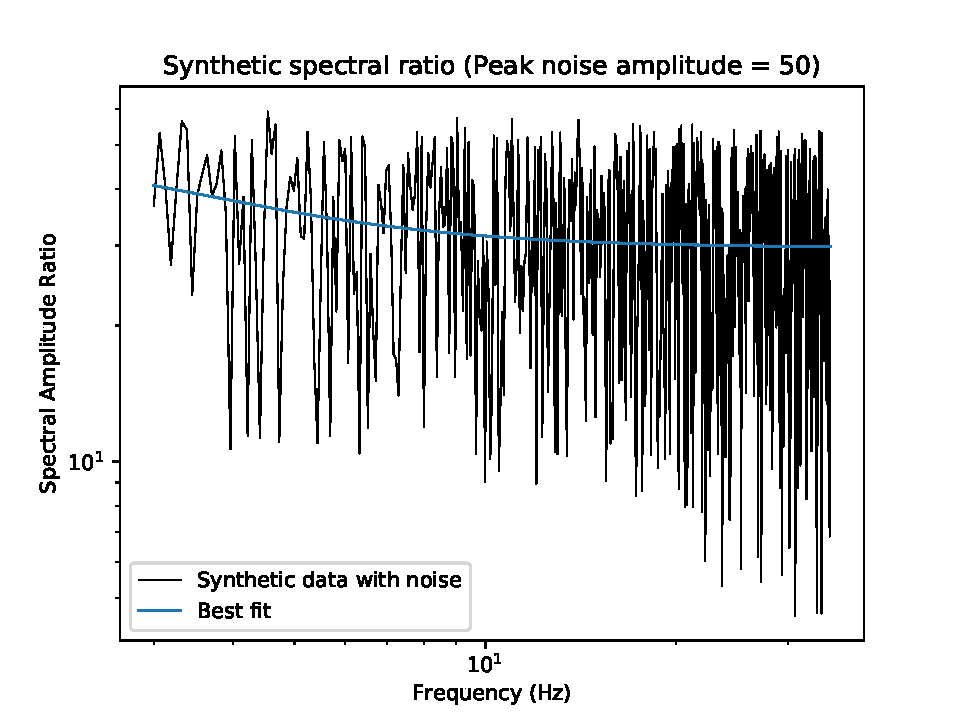
\includegraphics[scale=0.7]{fig_mom_noise_4.pdf}
    \caption{Synthetic spectral ratio with noise peak amplitude of 50.}
\end{figure}
\end{document}
